\documentclass{report}
\usepackage[english] {babel}

\usepackage{url}
\usepackage{cite}
\usepackage{graphicx}
\bibliographystyle{apalike}

\usepackage[section] {placeins}
\usepackage[a4paper, margin=0.7in] {geometry}
\setlength{\parindent}{0pt}
\setlength{\parskip}{5pt plus 2pt minus 1pt}

\title{Research Report}
\author{Thijs Boumans \and Patrick Kramer \and 
        Alexander Overvoorde \and Tim van Rossum}

\begin{document}
\maketitle

\begin{abstract}
	This report describes the problem of developing a collaborative augmented
	reality game. Each of the relevant technical details are analysed, like the
	AR glasses for local players, VR solution for external players and other
	components such as networking. This information is followed by proposed
	solutions for the actual gameplay, after which the final idea is chosen
	along with support for this choice. The report concludes with an overview
	of the game and technical details and how they will tie together for the
	final product.
\end{abstract}

\tableofcontents

\chapter{Problem Formulation} \label{cha:problem}
	% The problem description is taken from BEPSys. It has been shortened 
	% and slightly modified to fit the context of this document.
	While augmented reality research has grown into a mature field over the 
	last years, the aspects of situational awareness and presence of 
	augmented reality (AR) are still quite open research topics. This 
	project is about designing and implementing a collaborative game to 
	explore the different perception of situational awareness, presence and 
	workload in a physical and an AR environment. The game is to be employed 
	as an approximation of collaboratively solving complex problems, as they 
	occur in crime scene investigation when using virtual co-location, i.e. 
	expert remote crime scene investigators to guide local investigators in 
	AR to collaboratively analyse the crime scene. 
	
	It has to be possible to play the game with at least three players: At 
	least two players are present at the same location (physically 
	co-located). At least one player is physically remote but virtually 
	co-located \cite{bepsys}. The game itself should also be unable to be
	completed without either the physically co-located players or the 
	virtually co-located players, however this constraint could be relaxed
	to allow a higher playability of the game (because it would be nice to
	play the game without having to search for a virtually co-located player,
	for example).
	
	%TODO Add our interpretation to avoid ambiguities

\chapter{Problem Analysis} \label{cha:analysis}
	% Includes the challenges surrounding AR and Networking.
	% Also motivates the choices made.
	This chapter provides an analysis of the problem description of problems
	and challenges that may arise during development. It provides an analysis 
	of the problems and possible solutions that can be used in order to 
	solve these problems. 
	
	One of the core challenges of the project is the use of Augmented Reality 
	(AR) technology. An analysis of the available options to implement this 
	functionality is given in section \ref{sec:ar}. Another important challenge
	is improving situational awareness, which is discussed in section 
	\ref{sec:awareness}. The last challenge is the creation of interdependence 
	between players in such a way that requires collaboration from all players.
	This challenge is analyzed in section \ref{sec:interdependence}. 
	
	Lastly, a conclusion based on the analyses of these challenges is given in
	section \ref{sec:analysisconclusion}.
	
	\section{Augmented Reality (AR) Functionality} \label{sec:ar}
		% AR is a core element in the project. As such, we need to compare
		% various AR hardware devices and corresponding ways to implement
		% AR functionality for each device.
		Augmented Reality (AR) is a core aspect of the problem formulation. 
		As such, careful analysis has to be done as to how the AR functionality
		can be best implemented to fully address the context of this project.
		
		We consider two choices for implementing AR functionality: The META One,
		an optical see-through device (\ref{ssec:metaone}), and the Oculus Rift 
		Virtual Reality glasses in conjunction with mounted cameras 
		(\ref{ssec:oculusrift}).
	
		% Hardware devices to consider:
		\subsection{META One} \label{ssec:metaone}
			%   - META One (as indicated by the BEPSys project page)
			%       - Has a limited Field-of-View (around 35 degrees)
			%          - May interfere with the experience of the game.
			%       - Optical see-through glasses means AR works out of the box.
			
			The META One glasses are optical see-through glasses. Optical 
			see-through glasses work by projecting a virtual image on top of the
			world you see, effectively implementing a 3D AR exprience.
			
			Because the META One is an optical see-through device that also 
			features motion tracking, AR can be implemented simply by 
			projecting an image against a black background to the glasses.
			
			A big drawback of the available META One glasses is their 
			Field-of-View, which is 35 degrees. This Field-of-View is way lower
			than the Field-of-View of a person, which may have a negative impact 
			on the game experience.
			
		\subsection{Oculus Rift} \label{ssec:oculusrift}
			%   - Oculus Rift + mounted cameras (http://oculusvr.com/)
			%       - High Field-of-View (100 degrees)
			%       - VR glasses, so need to project the real world using cameras.
			%          - Limited resolution creates blurriness.
			%          - Projection can be done from within Unity
			%          - Potentially requires a lot of calibration
			% 		- Using Oculus Rift means we need to implement AR functionality 
			%         ourselves (as optical see-through often has this built-in).
			%         AR Libraries to consider:
			We've built a camera rig for the Oculus Rift that can be used to
			turn it into an augmented reality device. To detect the markers and
			render objects on them in Unity, there are several libraries
			available. Each of these will be discussed in the next sections.

			Oculus offers an SDK for Unity that makes it easy to integrate a
			game with the Rift. The challenge that we'll be facing during
			development is to properly integrate this SDK with the augmented
			reality libraries. Each of the frameworks try to take control of the
			camera in different ways and it's easy to get conflicts there.
			Getting the Rift see-through functionality working in Unity on its
			own and the augmented reality functionality on its own is not a
			challenge.

			\subsubsection{Vuforia} \label{sssec:vuforia}
				%   - Vuforia (http://vuforia.com/ and http://developer.vuforia.com/)
				%       - Includes integration with Unity
				Vuforia is a framework by Qualcomm that allows you to create
				arbitrary markers, import them into Unity and place objects onto
				them. You can then select a webcam and have it render the camera
				images with 3D objects projected onto the markers. It's very
				easy to use and has built-in support for virtual reality
				solutions like GearVR. The tracking quality is very good and
				stable, even with low quality markers (with few color transitions).

				Unfortunately it currently only works with the 32-bit version of
				Unity. It also lacks support for the Oculus Rift on the desktop,
				which means that we'll have to build that functionality ourselves.

			\subsubsection{Unity AR Toolkit (UART)} \label{sssec:uart}
				%   - Unity AR Toolkit (UART) (https://research.cc.gatech.edu/uart/content/contents/)
				%       - Source code and demos hosted on SourceForge (http://sourceforge.net/projects/uart/)
				%       - Seems to be a research project
				%       - Seems easy to use (comes with examples)
				%       - Built for Unity
				%       - Last change to SVN repo was in 2011.


			\subsubsection{Metaio} \label{sssec:metaio}
				%   - Metaio (http://www.metaio.com/)
				%       - Mainly oriented towards mobile phones, so may not be suitable for this project
	
		%   - ... <Add more as needed>
	
	\section{Situational Awareness} \label{sec:awareness}
		% Improving situational awareness is part of the main goal of the project.
		% We should indicate the steps needed to achieve this, which can be based 
		% on (possibly) a large range of scientific articles.
		This project is about exploring the different perception of situational 
		awareness, presence and workload in a physical and an AR environment 
		(see chapter \ref{cha:problem}). As such, situational awareness plays a 
		key role in this project.
		
	
	\section{Interdependence between players} \label{sec:interdependence}
		% Creating interdependence between players requires them to work together.
		% This can be done in several ways. We need to elaborate on the various ways
		% in which this can be achieved.
		The problem formulation states that the game is to be employed as an 
		approximation of collaboratively solving complex problems. In order to
		motivate players of the game to collaborate, there is a need to create
		a form of interdependence amongst the players. One way to do this is to 
		create an asymmetry between either the information that the players have or
		an asymmetry of abilities, as explained in the following subsection. 
		\subsection{Reasons to co-operate}
			The main reason to co-operate is the asymmetry of abilities between
			the players involved. For example: the physically co-located players
			have the ability to put down mirrors, and the virtually co-located
			players can then rotate the mirrors. Furthermore, information
			asymmetry can also be implemented, for example by allowing only the
			virtually co-located players to see the obstacles. Because of physical
			separation, asymmetry should be focused on physical abilities.
		
	\section{Virtual Co-location} \label{sec:virtualcolocation}
		Establishing virtual co-location is required to allow physically remote players
		to play the game together. As such, both the virtualization of the game world and
		the networking are considered in virtually co-locating physically remote players.
		Unity has multi player support, because of its master server to handle multi player
		games, but the server could be down at times. There are tutorials on the internet
		to create a basic multi player game that uses the master server to handle requests.
		These tutorials can be used to implement our own multilayer support. Alternatively
		we could provide the players with the means to easily get and exchange their IP
		addresses through other means such as mail. 
		Besides the networking we have to look at how we synchronize locations, depending on
		the chosen game we have in order of ascending complexity several options:
		1 Use markers with a known locations, this only works if we have a limited size 
		and reasonably fixed playing area which we can prepare ahead of time. This most 
		likely comes in the form of a set of markers at the edge and middle of the playing 
		field. 
		2 Use mobile markers which synchronize between players automatically, for example
		cards in a card game. This only works if we can trust the play er to keep these markers
		within their screen or if it does not matter if there is no augmentation needed if they
		cannot see a marker. 
		3 Object recognition which tracks the locations of objects in the scene,
		this method only works if there are a number of reasonably stable objects 
		within the player's vision. 
		4 Combining the output of a compass, a gyroscope and trilocations. This is 
		works regardless of what is visible but requires accurate trilocation which works
		can be quite hard to do without building a heavy rig. 
		Of course a combination of several of the above methods is also possible. 

		Then there is the matter of making the players "feel" that they are in the 
		same location. One obvious method might be to put an oculus on the remote player(s) and let 
		them see through the eyes of the local player(s), however this is likely to cause nausea. 
		Of course we can do away with the oculus but that might result in relative pasivism from 
		the remote players as they feel they cannot 
		even control their own view while not being forced to watch what the other player does. 

		We can also let the remote player control one or more avatars within the game world
		and view these through either oculus or screen. This would keep the remote player
		more interested by giving more of a feeling of agency then just viewing through the eyes 
		of the other player at the cost of the feeling of connectivity. But this would require 
		mapping out a large part of the scene in the virtual world. 
		
		Lastly we can also let the remote player view the world from a birds eye perspective 
		this can either be done by mounting a camera above the scene or by rendering it in 
		the virtual world, the second case offers increased player agency resulting in 
		a better attention to the situation at the cost of having the map the scene fully 
		in the virtual world. 
		
		% Allowing phsyically remote players to play the game, we need to establish
		% some idea of virtual co-location. This includes the virtualization of the 
		% game world as well as the networking functionality required to establish
		% the actual connection.
		
	\section{Analysis Conclusions} \label{sec:analysisconclusion}
		\section{Analysis Conclusions} \label{sec:analysisconclusion}
  % Provides the coices we made for the abovementioned problems along with a short
  % motivation based on the above analysis.
  
		% Provides the coices we made for the abovementioned problems along with a short
		% motivation based on the above analysis.

\chapter{Proposed Solutions} \label{cha:solution}
	% A description of the proposed solution, including gameplay elements.
	% The description is taken from the Product Plan. This section also
	% motivates why the proposed solution is a good solution.

\section{Laser mirror game} \label{sec:lasergame}
	The goal of the game is to solve a puzzle by controlling laser beams
	using mirrors in such a way that a predefined target is hit. The game
	can be played by one or more local players and one or more remote players.

	There are cards present for the local players that represent mirror
	bases. These must be placed on the table, which will be the locations
	for the mirrors. The local players will be able to see the mirrors they
	place through the use of AR technology. Each of the local players will
	only be given a few of the mirror bases needed to solve the puzzle, and
	as such solving the puzzle requires cooperation from all local players.

	The remote players can also see the placed mirrors, and can rotate them
	to influence the path of the laser beam(s). Only by cooperation between
	local players (who can only move the mirror bases) and remote players
	(who can only rotate them) it becomes possible to hit the target and as
	such solve the puzzle.

	The game provides various different types of mirrors with different
	properties, allowing for more complex puzzles. One example of such a
	mirror is a colored mirror, and then require the target is hit with the
	right (combination of) colors. Another way to make puzzles more complex
	is requiring that the players combine beams together to create more
	powerful beams. Other optical components like beam splitters can also be introduced.

	The game is designed to stimulate cooperation between the physically
	co-located players and the physically remote player(s). It does so by
	dividing abilities required for solving the puzzles amongst all players
	as follows:

	\begin{itemize}
		\item Physically co-located players each get only a part of the
		      mirror bases required to solve the puzzle, requiring input
		      from all of these players.
		\item If there are multiple virtually co-located players, each of
		      these players can only rotate a subset of the mirrors, and
		      as such input from all virtually co-located players is
		      required for solving the puzzle.
		\item Virtually co-located players have the ability to rotate
		      mirrors while the physically co-located players do not have
		      this ability, requiring input from both physically as well
		      as virtually co-located players.
	\end{itemize}

	Because of this division of abilities, there is an interdependence
	between all players (see section \ref{sec:interdependence}), regardless of
	whether these players are physically co-located or not. This replicates the
	interdependence that exists in the crime scene example as given in the
	problem formulation (see chapter \ref{cha:problem}).

\section{Platformer} \label{sec:platformer}
	The game starts with the avatar of the remote player appearing
	on the table and a goal appearing above the table. The local
  players have a pile of blocks, each of these blocks exists both
  in the virtual and real world.

	Inside the virtual world a number of pre-existing structures and
	obstacles exist making it harder for the remote player to move around.
	The local and remote player must work together in order to get the
	virtual avatar to the goal.

	Team work is heavily encouraged due to the interdependence between the
	players: There is information asymmetry (section \ref{ssec:information})
	because the remote player can see some pre-existing blocks the local
	player cannot see, and the fact that local players can place new blocks
	in the game world provides ability asymmetry (section \ref{ssec:ability}).

\section{FPS Survival game} \label{sec:fpssurvival}
	The goal of the game is to protect a virtual structure from enemies. These
	enemies will come from multiple sides to attack the structure while the
	remote players have to stop them. For doing so, they require the aid of the
	local players, who can place blocks (similar to the platformer game, section
	\ref{sec:platformer}) to block the path of the enemies.

	The local players can block the path of the enemies, but they cannot defeat
	them. The remote players, who view the game from a first-person perspective,
	have to defeat the enemies. Since the perspective of the remote players is
	limited (also partly because of the blocks placed by local players), they
	require information from the local players, who view the scene from above
	and as such have a good view of the entire situation. This creates
	information asymmetry between the players (section \ref{ssec:information}).

	To keep the game challenging, the enemies will grow stronger over time,
	requiring the cooperation between the local and remote players to improve
	as well. Because of the fact that local players can only defeat the enemies,
	and the remote players can block their path, there is a form of ability
	asymmetry between the local and remote players (section \ref{ssec:ability}).

\section{Tower defense} \label{sec:towerdefense}
	The local players start off with a number of towers each
	which have certain strengths and abilities. They must place
	these towers on a table in front of them. What they cannot
	but the remote player can see is what paths a number of
	hostile entities will take in order to attack their base.
	They must therefore cooperate to place the towers on the right
	positions to be able to defeat the enemies before they escape
	by communicating the ideal locations of the
	towers and paths that the hostile entities will take.

	This game idea is relatively simple, and because of the simplicity,
	complexity can easily be added to make the game more engaging. For
	example, towers could be upgradeable, utilizing resources that
	could be gained either by defeating individual enemies or by defeating
	a wave of enemies. These resources could then be used to upgrade
	tower types. As these resources are shared, and they can only be
	used once, players must work together to choose the best upgrade
	available in the given scenario. Enemies should also get procedurally
	stronger because of the increased capabilities of the towers.

	The problem with this idea is that it will very likely create a
	"puppet master" scenario where the remote player takes charge
	of the whole situation and the other players do not get a
	say in what is going to happen. This could be avoided by a
	number of extra abilities. This game shows heavy
	information and ability asymmetry.

\section{Minesweepers}
	This concept is based on the classic game of minesweeper. There's a grid
	where some of the squares have mines under them. Players each start at a
	random position and have to place flags on locations of mines while avoiding
	mines. The remote player is the only one who can see the numbers around
	squares, so he has to give instructions to the players on the field.

	The difference compared to the classic version of the game is that it's all
	physical. Local players walk around on the field, where they have to take
	careful steps to avoid triggering a mine. This turns the game into some sort
	of Twister variant where people can use special moves to quickly traverse
	the field and find all the mines. Local players co-operate by dividing the
	field into sections that they'll clear in parallel.

	The problem with this concept is the inherent *puppet master* phenomenon.
	Communication between the remote player and local players is very one-sided.
	Local players just receive commands where to step and where to plant flags
	and don't really have any input into the game themselves. Even if that
	problem was solved, the lack of cooperation aspects between local players
	would also be a big problem. Local players don't really have any reason to
	interact with each other. One way to solve that problem would be to require
	multiple players to place a flag.

	There are also some technical challenges with this concept. It requires that
	local players always know their exact position on a large field that they're
	inside of, which would require a lot of markers. Next, the position of their
	legs would have to be determined somehow to ensure that they're not stepping
	on a mine. Finally, a space large enough for a field would likely have to be
	found outside and sunlight doesn't play well with augmented reality devices.

\section{The chosen idea} \label{sec:chosenidea}
	The idea that is chosen is the mirror game idea. The reason for this
	decision is that it is a relatively simple idea, it can create hard
	to solve puzzles, and extra complexity can easily be added. It also
	prevents a "puppet master" scenario by giving both types of players
	about half of the abilities required for solving the game.

\chapter{Conclusion} \label{cha:conclusion}
In short, the mirror game seems the best solution to the problem. It is a viable project
to create in the given time frame, it is a challenging puzzle game even when playing a 
different version of it (a single-player version) on your own, and it taxes the communication
of both the remote and the local players, as they both have abilities necessary for
achieving the goal, but they cannot achieve it on their own (although this could be relaxed
to make the game more playable). Also, it is still a challenging project, because of the
technical challenge of integrating AR hardware and recognition of markers with the game
world. Additional complexity, such as colored laser beams/targets, beam splitters, beam mergers
etc. could also be implemented to increase the technical challenge of the problem.

The game and networking will be implemented using Unity, with the Vuforia library
handling augmented reality for the local players. The remote players will likely
be using an Oculus Rift and the local players one of the augmented reality devices
describes in the problem analysis that ends up working best in practice.
	% Summarizes the Research Report and provides 
	% an overview and conclusion of the technologies 
	% we're going to use.
	% TODO AR tech elaboration.	

Using this information, we've built a small demo that uses Vuforia. It places
a laser emitter, mirror and wall on three markers that can be moved around. The
mirror reflects the laser realistically based on the angle of incidence.

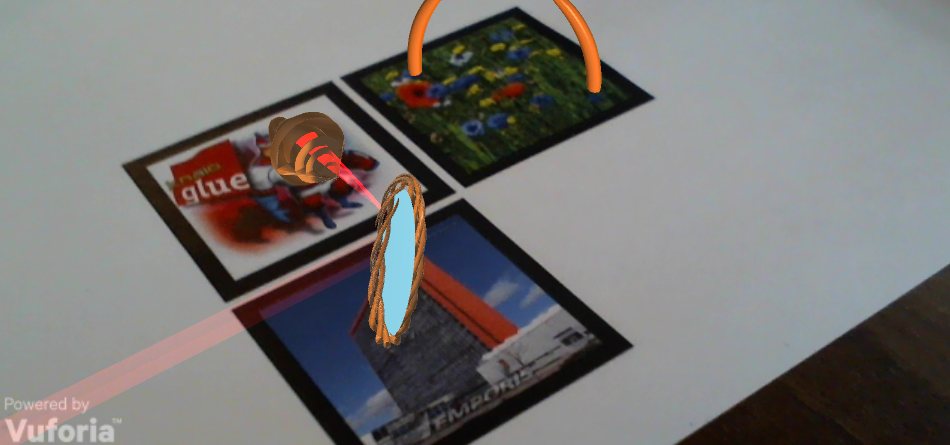
\includegraphics[scale=0.7]{demo.png}

\pagebreak % Required to fix page numbering in Table of Contents
\bibliography{Bibliography}
\addcontentsline{toc}{chapter}{Bibliography}

\end{document}
